\cleardoubleoddpage
\begingroup
\fontsize{11pt}{13.2pt}\selectfont
\chapter{Methodology}
\label{chap:methodology}

This chapter develops the methodological framework for both experimental tracks. We formalise the out-of-distribution detection problem as a binary generative classification task, introduce the class-conditional separation loss that is the primary novel contribution of this work, and describe the two-stage inkjet quality control pipeline with its multi-head conditional diffusion model. Formal analysis and architectural details are provided throughout to ground the experimental choices made in Chapters~\ref{chap:implementation} and~\ref{chap:results}.


\section{Problem Formulation}
\label{sec:meth:problem}

This section formalises the OOD detection problem and establishes how conditional diffusion models can be used as generative classifiers for this task.

\subsection{Relation to One-Class Novelty Detection}
\label{sec:meth:problem:oneclass}

Our problem formulation differs from the standard multi-class OOD detection benchmark setting. In the standard protocol (e.g., OpenOOD~\cite{zhang2023openood}), a multi-class classifier is trained on all classes of an in-distribution dataset (e.g., all 10 CIFAR-10 classes), and OOD detection is evaluated on samples from entirely different datasets. By contrast, our binary CDM models a single target class (airplane) against all others, which is closer to the one-class novelty detection (also called one-class classification or anomaly detection) paradigm~\cite{ruff2018deep, tack2020csi}.

In one-class novelty detection, a model learns the distribution of a single ``normal'' class and flags deviations as anomalous. Classical approaches include One-Class SVM~\cite{scholkopf2001estimating}, Deep SVDD~\cite{ruff2018deep}, and contrastive methods such as CSI~\cite{tack2020csi} and PANDA~\cite{reiss2021panda}. Our binary CDM extends this paradigm by explicitly modelling both the target class and an OOD proxy class, enabling contrastive scoring rather than relying on a single normality model. This dual-condition design is the key architectural distinction from pure one-class methods and is what enables the separation loss to amplify the reconstruction gap.

Consequently, direct numerical comparison with standard multi-class OOD benchmarks (MSP, ODIN, Energy on all-class CIFAR-10) would be misleading, as they solve a different problem. Instead, we contextualise our results against one-class baselines evaluated on the same per-class CIFAR-10 protocol in Section~\ref{sec:results:baselines}.

\subsection{Mathematical Definition}
\label{sec:meth:problem:math}

With the general OOD detection formulation established in Chapter~\ref{chap:background}, we now focus on our approach using conditional diffusion models.

\textbf{Binary Training Setup:} We assume access to a labelled training dataset $\mathcal{D}_{\text{train}} = \{(x_i, y_i)\}_{i=1}^{n}$ where $x_i \in \mathbb{R}^{3 \times 32 \times 32}$ are CIFAR-10 images and $y_i \in \{0, 1\}$ are binary labels: $y = 0$ for the in-distribution class (airplane, CIFAR-10 class~0) and $y = 1$ for the OOD-proxy class (all other nine CIFAR-10 classes pooled together). The data is drawn i.i.d.\ from the training distribution $P_{\text{train}}(x, y)$. Consistent with the OOD-positive scoring convention stated in Section~\ref{sec:bg:ood:problem}, higher values of the scoring function $s_{\text{OOD}}(x)$ indicate greater evidence of being out-of-distribution.

\textbf{Test Setup:} At test time, we receive samples $x_{\text{test}}$ from either:
\begin{itemize}
    \item \textbf{In-distribution (ID):} $x_{\text{test}} \sim p(x \mid y = 0)$, i.e.\ airplane images.
\item \textbf{OOD:} $x_{\text{test}} \sim P_{\text{ood}}(x)$, where $P_{\text{ood}}$ is either the within-CIFAR OOD proxy ($y = 1$ pool) or an unseen external dataset. In the external benchmark protocol, these external samples are evaluated against the full CIFAR-10 test reference pool because the binary CDM was trained on both conditional branches of CIFAR-10 (airplane as $c{=}0$, non-airplane as $c{=}1$). The core reproducible external set comprises CIFAR-100, Places365, FashionMNIST, SVHN, and Textures.
\end{itemize}

\textbf{Binary Generative Classification Framework:} We train a single conditional diffusion model to learn the two class-conditional distributions $p_\theta(x \mid c)$ for $c \in \{0, 1\}$. (Here and throughout, $c$ denotes the binary class condition, generalising the training label $y$: $c = 0$ refers to the ID class and $c = 1$ to the OOD-proxy class.) For OOD detection we exploit the observation that ID samples should be reconstructed accurately under the ID condition ($c = 0$) but poorly under the OOD condition ($c = 1$), and vice versa for OOD samples.

\textbf{Per-Condition Reconstruction Errors:} For a test sample $x$ we compute reconstruction errors under each condition:

\begin{equation}
\label{eq:meth:e0}
e_0(x) = \mathbb{E}_{t \sim \mathcal{U}[1,T],\, \epsilon \sim \mathcal{N}(0,I)} \left[ \left\| \epsilon - \epsilon_\theta\!\left( \sqrt{\bar{\alpha}_t}\, x + \sqrt{1 - \bar{\alpha}_t}\, \epsilon,\, t,\, c{=}0 \right) \right\|^2 \right]
\end{equation}

\begin{equation}
\label{eq:meth:e1}
e_1(x) = \mathbb{E}_{t \sim \mathcal{U}[1,T],\, \epsilon \sim \mathcal{N}(0,I)} \left[ \left\| \epsilon - \epsilon_\theta\!\left( \sqrt{\bar{\alpha}_t}\, x + \sqrt{1 - \bar{\alpha}_t}\, \epsilon,\, t,\, c{=}1 \right) \right\|^2 \right]
\end{equation}

where $\epsilon_\theta(x_t, t, c)$ is the noise-prediction UNet conditioned on binary class $c$.

\textbf{OOD Scoring Function (Difference):} The primary scoring method computes the signed difference between ID-conditioned and OOD-conditioned errors:

\begin{equation}
\label{eq:meth:sood}
s_{\text{OOD}}(x) = e_0(x) - e_1(x)
\end{equation}

A high score indicates the model denoises $x$ far better under the OOD condition than the ID condition, which is strong evidence that $x$ is out-of-distribution. Samples with $s_{\text{OOD}}(x) > \tau$ (for threshold $\tau$) are classified as OOD.

\textbf{Alternative Scoring Methods:} We also investigate:

\begin{equation}
\label{eq:meth:sratio}
s_{\text{ratio}}(x) = \frac{e_0(x)}{e_1(x)}
\end{equation}

\begin{equation}
\label{eq:meth:sidonly}
s_{\text{id-only}}(x) = e_0(x)
\end{equation}

The ratio formulation normalises by the magnitude of the OOD-conditioned error, making it more robust to scale differences across OOD distributions. The ID-only formulation ignores the OOD-conditioned error entirely; we include it as an ablation to measure the contribution of contrastive scoring. Section~\ref{sec:results:ablations} shows that comparing the two conditional errors (difference or ratio) is essential: ID-only scoring collapses to 20.2\% AUROC on SVHN.

\subsection{OOD Scoring Algorithm}
\label{sec:meth:problem:algorithm}

Algorithm~1 details the procedure for computing OOD scores at inference time.

\medskip
\noindent\rule{\textwidth}{0.4pt}
\smallskip
\begin{minipage}{\linewidth}\small\sloppy
\noindent\textbf{Algorithm 1} \emph{Binary CDM OOD Scoring (Difference Method).}\label{alg:ood_evaluation}

\noindent\textbf{Require:} Test image $x \in \mathbb{R}^{3 \times 32 \times 32}$, trained model $\epsilon_\theta$\\
\textbf{Require:} Number of MC trials $K$, timesteps $T$, threshold $\tau$\\
\textbf{Ensure:} OOD score $s(x)$, decision $\text{is\_ood} \in \{0, 1\}$

\noindent
1:\ $\hat{e}_0 \leftarrow 0$;\ $\hat{e}_1 \leftarrow 0$\\
2:\ \textbf{for} trial $k = 1$ to $K$ \textbf{do}\\
3:\quad $t_k \sim \text{Uniform}\{1, \ldots, T\}$;\ $\epsilon_k \sim \mathcal{N}(0, I)$\\
4:\quad $x_{t_k} \leftarrow \sqrt{\bar{\alpha}_{t_k}}\, x + \sqrt{1 - \bar{\alpha}_{t_k}}\, \epsilon_k$\\
5:\quad $\hat{e}_0 \leftarrow \hat{e}_0 + \|\epsilon_k - \epsilon_\theta(x_{t_k}, t_k, c{=}0)\|^2$\\
6:\quad $\hat{e}_1 \leftarrow \hat{e}_1 + \|\epsilon_k - \epsilon_\theta(x_{t_k}, t_k, c{=}1)\|^2$\\
7:\ \textbf{end for}\\
8:\ $\hat{e}_0 \leftarrow \hat{e}_0 / K$;\ $\hat{e}_1 \leftarrow \hat{e}_1 / K$\\
9:\ $s(x) \leftarrow \hat{e}_0 - \hat{e}_1$ (positive: OOD; negative: ID)\\
10:\ \textbf{if} $s(x) > \tau$ \textbf{then return} OOD \textbf{else return} ID
\end{minipage}
\smallskip
\noindent\rule{\textwidth}{0.4pt}
\medskip

\textbf{Complexity Analysis:} The cost of Algorithm~1 is $O(2K \cdot N)$ where $N$ is the cost of one forward pass. For $K = 50$ and the binary UNet (${\approx}68.8$M parameters), the measured timing is 4861.1\,s (about 81.0 minutes) per 10{,}000 images on an NVIDIA GeForce RTX 2080 Ti, roughly $492\times$ the wall-clock cost of a ResNet-18 forward pass on the same hardware. Section~\ref{sec:results:ablations} shows that $K = 10$ reduces this to 972.9\,s (about 16.2 minutes; $68.6\times$ ResNet-18 cost) while achieving 98.2\% AUROC, close to the 98.6\% at $K = 50$.

\textbf{Threshold Calibration:} The threshold $\tau$ is calibrated on a validation set to achieve a target false positive rate (typically 5\%). We set $\tau$ to the $(1 - \text{FPR}_{\text{target}})$-th quantile of $s_{\text{OOD}}$ scores computed on ID validation samples.


\subsection{Evaluation Metrics}
\label{sec:meth:problem:metrics}

Following standard practice in OOD detection, we evaluate our methods using three primary metrics:

\textbf{Area Under the ROC Curve (AUROC):} The ROC curve plots the True Positive Rate (TPR) against the False Positive Rate (FPR) as the threshold $\tau$ varies:

\begin{equation}
\label{eq:meth:tpr}
\text{TPR}(\tau) = P_{x \sim P_{\text{ood}}}\!\left[s_{\text{OOD}}(x) > \tau\right]
\end{equation}

\begin{equation}
\label{eq:meth:fpr}
\text{FPR}(\tau) = P_{x \sim P_{\text{id}}}\!\left[s_{\text{OOD}}(x) > \tau\right]
\end{equation}

The AUROC measures the probability that a randomly chosen OOD sample has a higher score than a randomly chosen ID sample:

\begin{equation}
\label{eq:meth:auroc}
\text{AUROC} = P_{x_{\text{OOD}} \sim P_{\text{ood}},\, x_{\text{ID}} \sim P_{\text{id}}}\!\left[s_{\text{OOD}}(x_{\text{OOD}}) > s_{\text{OOD}}(x_{\text{ID}})\right]
\end{equation}

An AUROC of 1.0 indicates perfect separation, while 0.5 indicates random guessing. Higher values are better.

\textbf{False Positive Rate at 95\% TPR (FPR@95\%TPR):} This metric measures the fraction of ID samples incorrectly flagged as OOD when the threshold is set such that 95\% of OOD samples are correctly detected:

\begin{equation}
\label{eq:meth:fprtpr95}
\text{FPR@95\%TPR} = \text{FPR}(\tau^*) \quad\text{where}\quad \tau^* = \sup\!\left\{\tau : \text{TPR}(\tau) \geq 0.95\right\}
\end{equation}

This metric is particularly important for safety-critical applications where we must detect most OOD samples while minimising false alarms. Lower values are better.

\textbf{Balanced Detection Accuracy:} The balanced accuracy at an optimal threshold (chosen to maximise Youden's $J$ statistic):

\begin{equation}
\label{eq:meth:balanced}
\text{Balanced Accuracy} = \max_\tau \left[ \tfrac{1}{2}\,\text{TPR}(\tau) + \tfrac{1}{2}\left(1 - \text{FPR}(\tau)\right) \right]
\end{equation}

We also report Area Under the Precision-Recall Curve (AUPRC) and Detection Error (average of false positive and false negative rates) for thorough evaluation.


\section{Diffusion Models for OOD Detection}
\label{sec:meth:diffusion}

This section provides the theoretical foundation for using diffusion models for OOD detection and formalises why reconstruction error serves as an effective OOD signal.

\subsection{Theoretical Foundation}
\label{sec:meth:diffusion:theory}

\textbf{Why Diffusion Models for OOD Detection?}
Diffusion models offer several advantages for OOD detection that address limitations of previous approaches.

First, they provide a reconstruction-based alternative to direct likelihood estimation. As discussed in Section~\ref{sec:bg:manifold}, likelihood-based OOD detection can fail in high dimensions because likelihood is affected by both density and ambient volume. Instead of computing $p(x)$ directly, we measure reconstruction error, which approximates the distance from $x$ to the learnt data support. The denoising process can be viewed as a projection operator:

\begin{equation}
\label{eq:meth:projection}
\pi_\theta(x) = \mathbb{E}[x_0 \mid x_T = x + \text{noise}]
\end{equation}

where $x_0$ is the denoised reconstruction. The reconstruction error $\|x - \pi_\theta(x)\|$ provides a distance-like measure to the learnt manifold.

Second, unlike VAEs that decode in a single step, diffusion models iteratively refine over $T$ steps, providing multiple opportunities to accumulate evidence about whether a sample fits the learnt distribution~\cite{wyatt2022anoddpm, graham2023denoising}. Each denoising step $x_t \to x_{t-1}$ can be viewed as a gradient step towards high-density regions.

Third, diffusion models enjoy stable training: they avoid the mode collapse of generative adversarial networks (GANs) and the posterior collapse of VAEs, relying only on a simple mean squared error (MSE) objective.

Fourth, class-conditional density modelling allows the network to learn separate denoising pathways per class, effectively modelling $p_\theta(x \mid y)$ for each $y \in \mathcal{Y}$. This enables fine-grained OOD detection: we can measure the fit of a test sample to each known class individually.

\subsection{Reconstruction Error as OOD Signal}
\label{sec:meth:diffusion:signal}

We now formalise why reconstruction error from diffusion models provides an effective OOD signal.

\textbf{Low-Dimensional Support Perspective:} If class-conditional image data concentrate near lower-dimensional supports (Section~\ref{sec:bg:manifold}), the conditional diffusion model learns to approximate these structures $\mathcal{M}_c$ for each class $c$. For an ID sample $x \sim p(x \mid y = c)$, the sample lies on or near $\mathcal{M}_c$ and the denoising process recovers $x$ with low error. For an OOD sample $x \sim P_{\text{ood}}$, the sample lies far from all learnt supports, and denoising projects $x$ towards the nearest learnt support, incurring high reconstruction error.

\textbf{Score-Based Interpretation:} Recall from Section~\ref{sec:bg:diffusion} that the noise prediction network approximates the score function:

\begin{equation}
\label{eq:meth:score_interp}
\epsilon_\theta(x_t, t, c) \approx -\sqrt{1 - \bar{\alpha}_t}\, \nabla_{x_t} \log p(x_t \mid y = c)
\end{equation}

The reconstruction error in Equations~\ref{eq:meth:e0}--\ref{eq:meth:e1} thus measures how well $x$ aligns with the learnt score function for class $c$. Samples that require large score corrections (high error) are likely OOD.

\textbf{Empirical Risk Minimisation Perspective:} During training, the model minimises:

\begin{equation}
\label{eq:meth:class_loss}
\mathcal{L}_c = \mathbb{E}_{x \sim p(x|y=c),\, t,\, \epsilon} \left[ \left\| \epsilon - \epsilon_\theta\!\left( \sqrt{\bar{\alpha}_t}\, x + \sqrt{1 - \bar{\alpha}_t}\,\epsilon,\, t,\, c \right) \right\|^2 \right]
\end{equation}

For test samples $x$ from $p(x \mid y = c)$, we expect $e_c(x) \approx \mathcal{L}_c$ (low, when $c$ is the correct class condition for $x$). For OOD samples, there is a distribution mismatch, leading to $e_c(x) \gg \mathcal{L}_c$ (high).

\textbf{Information-Theoretic View:} The reconstruction error can be interpreted as a measure of the information content needed to correct the model's predictions. ID samples require little correction information (they fit the model's learnt patterns), while OOD samples require substantial correction (they deviate from learnt patterns).

\textbf{Relation to the Likelihood Pitfall.} The key difference from likelihood-based methods is that reconstruction error measures distance in the learnt representation space, not volume in the ambient space~\cite{kirichenko2020why, fefferman2016manifold}. While a high-dimensional OOD manifold might have more ambient volume than a low-dimensional ID manifold (causing likelihood to fail), it cannot have systematically lower reconstruction error when trained only on ID data. The diffusion model's denoising pathways are optimised specifically for ID manifolds, making OOD samples difficult to reconstruct accurately.

\subsection{Heuristic Analysis of Reconstruction Error Separation}
\label{sec:meth:diffusion:formal}

We now provide a heuristic analysis establishing conditions under which reconstruction error separates ID from OOD samples. The following statements are motivational rather than fully proved: Informal Argument~1 is a standard bias--variance decomposition and Informal Claim~2 is grounded in the training objective. A rigorous treatment would require explicit assumptions on support geometry, noise-schedule dependence, and Lipschitz regularity of the score function, which we leave as future theoretical work.

\textbf{Setup.} Let $\mathcal{M}_{\text{ID}} \subset \mathbb{R}^D$ denote the support of the in-distribution, and let $\epsilon^*(x_t, t, c)$ denote the Bayes-optimal denoiser for class $c$, which minimises the expected MSE over the class-conditional distribution. The trained model $\epsilon_\theta$ approximates $\epsilon^*$ with approximation error $\delta_\theta = \mathbb{E}[\|\epsilon_\theta - \epsilon^*\|^2]$.

\textbf{Informal Argument 1} \emph{(Standard MSE decomposition; ID reconstruction error bound).} \textit{Assuming $x$ is drawn i.i.d.\ from the class-conditional training distribution, the Bayes-optimal denoiser is evaluated under the same noising process as training, and the learnt denoiser has approximation gap $\delta_\theta$, the expected reconstruction error under the correct class condition satisfies:}

\begin{equation}
\label{eq:meth:id_bound}
\mathbb{E}_{t,\epsilon} \left[ \left\| \epsilon - \epsilon_\theta(x_t, t, c) \right\|^2 \right] \leq \mathcal{L}_c^* + \delta_\theta
\end{equation}

where $\mathcal{L}_c^* = \mathbb{E}_{x \sim p(x|c),\, t,\, \epsilon}[\|\epsilon - \epsilon^*(x_t, t, c)\|^2]$ is the irreducible Bayes error for class $c$, and $\delta_\theta$ is the model's approximation gap.

\textbf{Justification.} This follows from the Pythagorean decomposition of MSE: for any estimator $\epsilon_\theta$, $\mathbb{E}[\|\epsilon - \epsilon_\theta\|^2] = \mathbb{E}[\|\epsilon - \epsilon^*\|^2] + \mathbb{E}[\|\epsilon^* - \epsilon_\theta\|^2]$. The Bayes-optimal denoiser achieves $\mathcal{L}_c^*$ on in-distribution data, and the learnt model adds at most $\delta_\theta$ additional error due to finite capacity and training.

\textbf{Informal Claim 2} \emph{(OOD reconstruction error lower bound).} \textit{Assuming the OOD sample lies outside the support on which the class-conditional denoiser was optimised, the denoiser is locally regular rather than adversarially extrapolating, and the selected timestep range preserves information about the support mismatch, an OOD sample $x_{\text{ood}}$ at support distance $d(x_{\text{ood}}, \mathcal{M}_c) = \inf_{x' \in \mathcal{M}_c} \|x_{\text{ood}} - x'\|$ satisfies:}

\begin{equation}
\label{eq:meth:ood_bound}
\mathbb{E}_{t,\epsilon} \left[ \left\| \epsilon - \epsilon_\theta(x_t^{\text{ood}}, t, c) \right\|^2 \right] \geq \mathcal{L}_c^* + \Delta_{\text{ood}}(d)
\end{equation}

where $\Delta_{\text{ood}}(d) > 0$ is a distribution mismatch term that is monotonically increasing in $d(x_{\text{ood}}, \mathcal{M}_c)$ for sufficiently large $d$.

\textbf{Justification.} The denoiser $\epsilon_\theta$ is trained to minimise error over $p(x \mid c)$. When evaluated on $x_{\text{ood}} \notin \text{supp}(p(x \mid c))$, the noised input $x_t^{\text{ood}}$ falls in a region of the noised space where the denoiser has not been optimised. For small noise levels ($t \ll T$), $x_t^{\text{ood}}$ remains close to $x_{\text{ood}}$ and thus far from the noised ID manifold, yielding large prediction error. For large noise levels ($t \approx T$), both ID and OOD samples converge to isotropic Gaussian noise, reducing the gap. The expected mismatch $\Delta_{\text{ood}}$ thus depends on both the manifold distance $d$ and the timestep distribution used for scoring.

\textbf{Corollary} \emph{(Separation condition).} \textit{OOD detection via reconstruction error succeeds when:}

\begin{equation}
\label{eq:meth:sep_condition}
\Delta_{\text{ood}}(d) > \delta_\theta + \operatorname{Var}[e_{\text{ID}}]
\end{equation}

where $\operatorname{Var}[e_{\text{ID}}]$ is the variance of reconstruction error across ID samples. In words: the distribution mismatch must exceed the sum of model approximation error and natural ID variation.

\textbf{Connection to Empirical Observations.} This analysis explains several empirical findings:
\begin{itemize}
    \item \textbf{Near-OOD vs.\ far-OOD detection difficulty:} In the reproducible core results, CIFAR-100 (a near-OOD dataset sharing low-level visual statistics with CIFAR-10) achieves higher AUROC (96.97\%) than far-OOD datasets such as Textures (92.84\%) and FashionMNIST (94.03\%). This occurs because CIFAR-100's airplane class is under-represented, creating a distributional gap that the model exploits effectively, which shows that semantic proximity does not deterministically predict detection difficulty.
    \item \textbf{Uniform timestep sampling is the best-tested strategy:} Averaging over all $t$ captures both the high-sensitivity regime ($t \ll T$, where OOD deviation is maximal) and moderate-noise levels, maximising effective $\Delta_{\text{ood}}$. Section~\ref{sec:results:ablations} confirms that restricting to mid-range timesteps ($t \in [250, 750]$) reduces SVHN AUROC by 1.6\%.
    \item \textbf{Separation loss improves both mean AUROC and stability:} The binary conditioning structure ($c{=}0$ for airplane, $c{=}1$ for all others) gives the model two class-conditional denoising paths. With binary conditioning but no separation loss ($\lambda = 0$), the three-seed Within-CIFAR mean is $92.52\% \pm 11.07\%$; adding the separation loss ($\lambda = 0.02$) raises the mean to $99.03\% \pm 0.07\%$ and largely removes the seed sensitivity.
\end{itemize}

\textbf{Limitations.} This analysis relies on several simplifying assumptions: (i) the ID distribution is concentrated near a learnable lower-dimensional support, (ii) the model's approximation error $\delta_\theta$ is small relative to the distribution mismatch, and (iii) the OOD distribution does not happen to lie in a region where the denoiser generalises well despite never training there. Assumption~(iii) can fail for adversarially constructed OOD inputs. Formalising these bounds with explicit dependence on $D$, $T$, and support geometry remains an open theoretical challenge.


\section{Model Architectures}
\label{sec:meth:architectures}

We use a conditional diffusion model for OOD detection and then describe the multi-condition architecture used for the inkjet quality control application.

\subsection{Conditional Diffusion Model}
\label{sec:meth:architectures:cdm}

Our primary approach uses a conditional diffusion model that learns class-specific denoising processes.

\textbf{Architecture:} We employ a UNet-based architecture with the following components:
\begin{itemize}
    \item \textbf{Encoder:} Downsampling path with residual blocks and self-attention at resolution $8 \times 8$
    \item \textbf{Bottleneck:} Multiple residual blocks with self-attention for capturing global context
    \item \textbf{Decoder:} Upsampling path with skip connections from encoder
    \item \textbf{Class Conditioning:} Learnt class embeddings $e_y \in \mathbb{R}^{d_{\text{emb}}}$ added to timestep embeddings
    \item \textbf{Timestep Embedding:} Sinusoidal positional encoding of timestep $t$
\end{itemize}

\textbf{Mathematical Formulation:} The network predicts noise conditioned on both timestep $t$ and class $y$:

\begin{equation}
\label{eq:meth:unet_formulation}
\epsilon_\theta(x_t, t, y) = \text{UNet}\!\left(x_t,\, \text{TimeEmbed}(t) + \text{ClassEmbed}(y)\right)
\end{equation}

where $\text{TimeEmbed} : \{1, \ldots, T\} \to \mathbb{R}^{d_{\text{emb}}}$ and $\text{ClassEmbed} : \{1, \ldots, C\} \to \mathbb{R}^{d_{\text{emb}}}$ are learnt embedding functions.

\textbf{Training:} Following classifier-free guidance, we randomly drop the class conditioning with probability $p_{\text{uncond}} = 0.1$ during training:

\begin{equation}
\label{eq:meth:cfg_training}
\mathcal{L} = \mathbb{E}_{x,y,t,\epsilon} \left[ \left\| \epsilon - \epsilon_\theta\!\left( \sqrt{\bar{\alpha}_t}\, x + \sqrt{1 - \bar{\alpha}_t}\,\epsilon,\, t,\, y' \right) \right\|^2 \right]
\end{equation}

where $y' = y$ with probability $1 - p_{\text{uncond}}$ and $y' = \varnothing$ (null class) with probability $p_{\text{uncond}}$. This enables the model to perform both conditional and unconditional denoising.

\textbf{OOD Detection:} For a test sample $x$, we compute reconstruction error for each class:

\begin{equation}
\label{eq:meth:ec_estimate}
\hat{e}_c(x) = \frac{1}{K} \sum_{k=1}^{K} \left\| \epsilon_k - \epsilon_\theta\!\left( \sqrt{\bar{\alpha}_{t_k}}\, x + \sqrt{1 - \bar{\alpha}_{t_k}}\, \epsilon_k,\, t_k,\, c \right) \right\|^2
\end{equation}

where we sample $K$ random timesteps $t_k \sim \mathcal{U}[1, T]$ and noise vectors $\epsilon_k \sim \mathcal{N}(0, I)$ to obtain a Monte Carlo estimate of the population error $e_c(x)$. The OOD score is then computed by substituting $\hat{e}_0(x)$ and $\hat{e}_1(x)$ into Equation~\ref{eq:meth:sood}.

\textbf{Design Rationale:} The conditional model can learn class-specific patterns. ID samples from class $c$ should be well-reconstructed using the $c$-conditioned denoising path but poorly reconstructed using other class paths. OOD detection therefore uses the contrastive score in Equation~\ref{eq:meth:sood}, comparing reconstruction errors under the ID and auxiliary non-ID conditions rather than relying on a minimum-error rule.


\section{Inkjet Quality Control Pipeline}
\label{sec:meth:inkjet}

This section describes the two-stage pipeline for inkjet print quality classification using conditional diffusion models, which serves as a practical application of the generative classification principles developed above.

\subsection{Two-Stage Pipeline Overview}
\label{sec:meth:inkjet:overview}

Our pipeline processes full template images ($1920 \times 1080$ pixels) of inkjet prints through two sequential stages: (1)~feature detection using YOLOv8, and (2)~quality classification using a conditional diffusion model (CDM).

\begin{figure}[htbp]
    \centering
    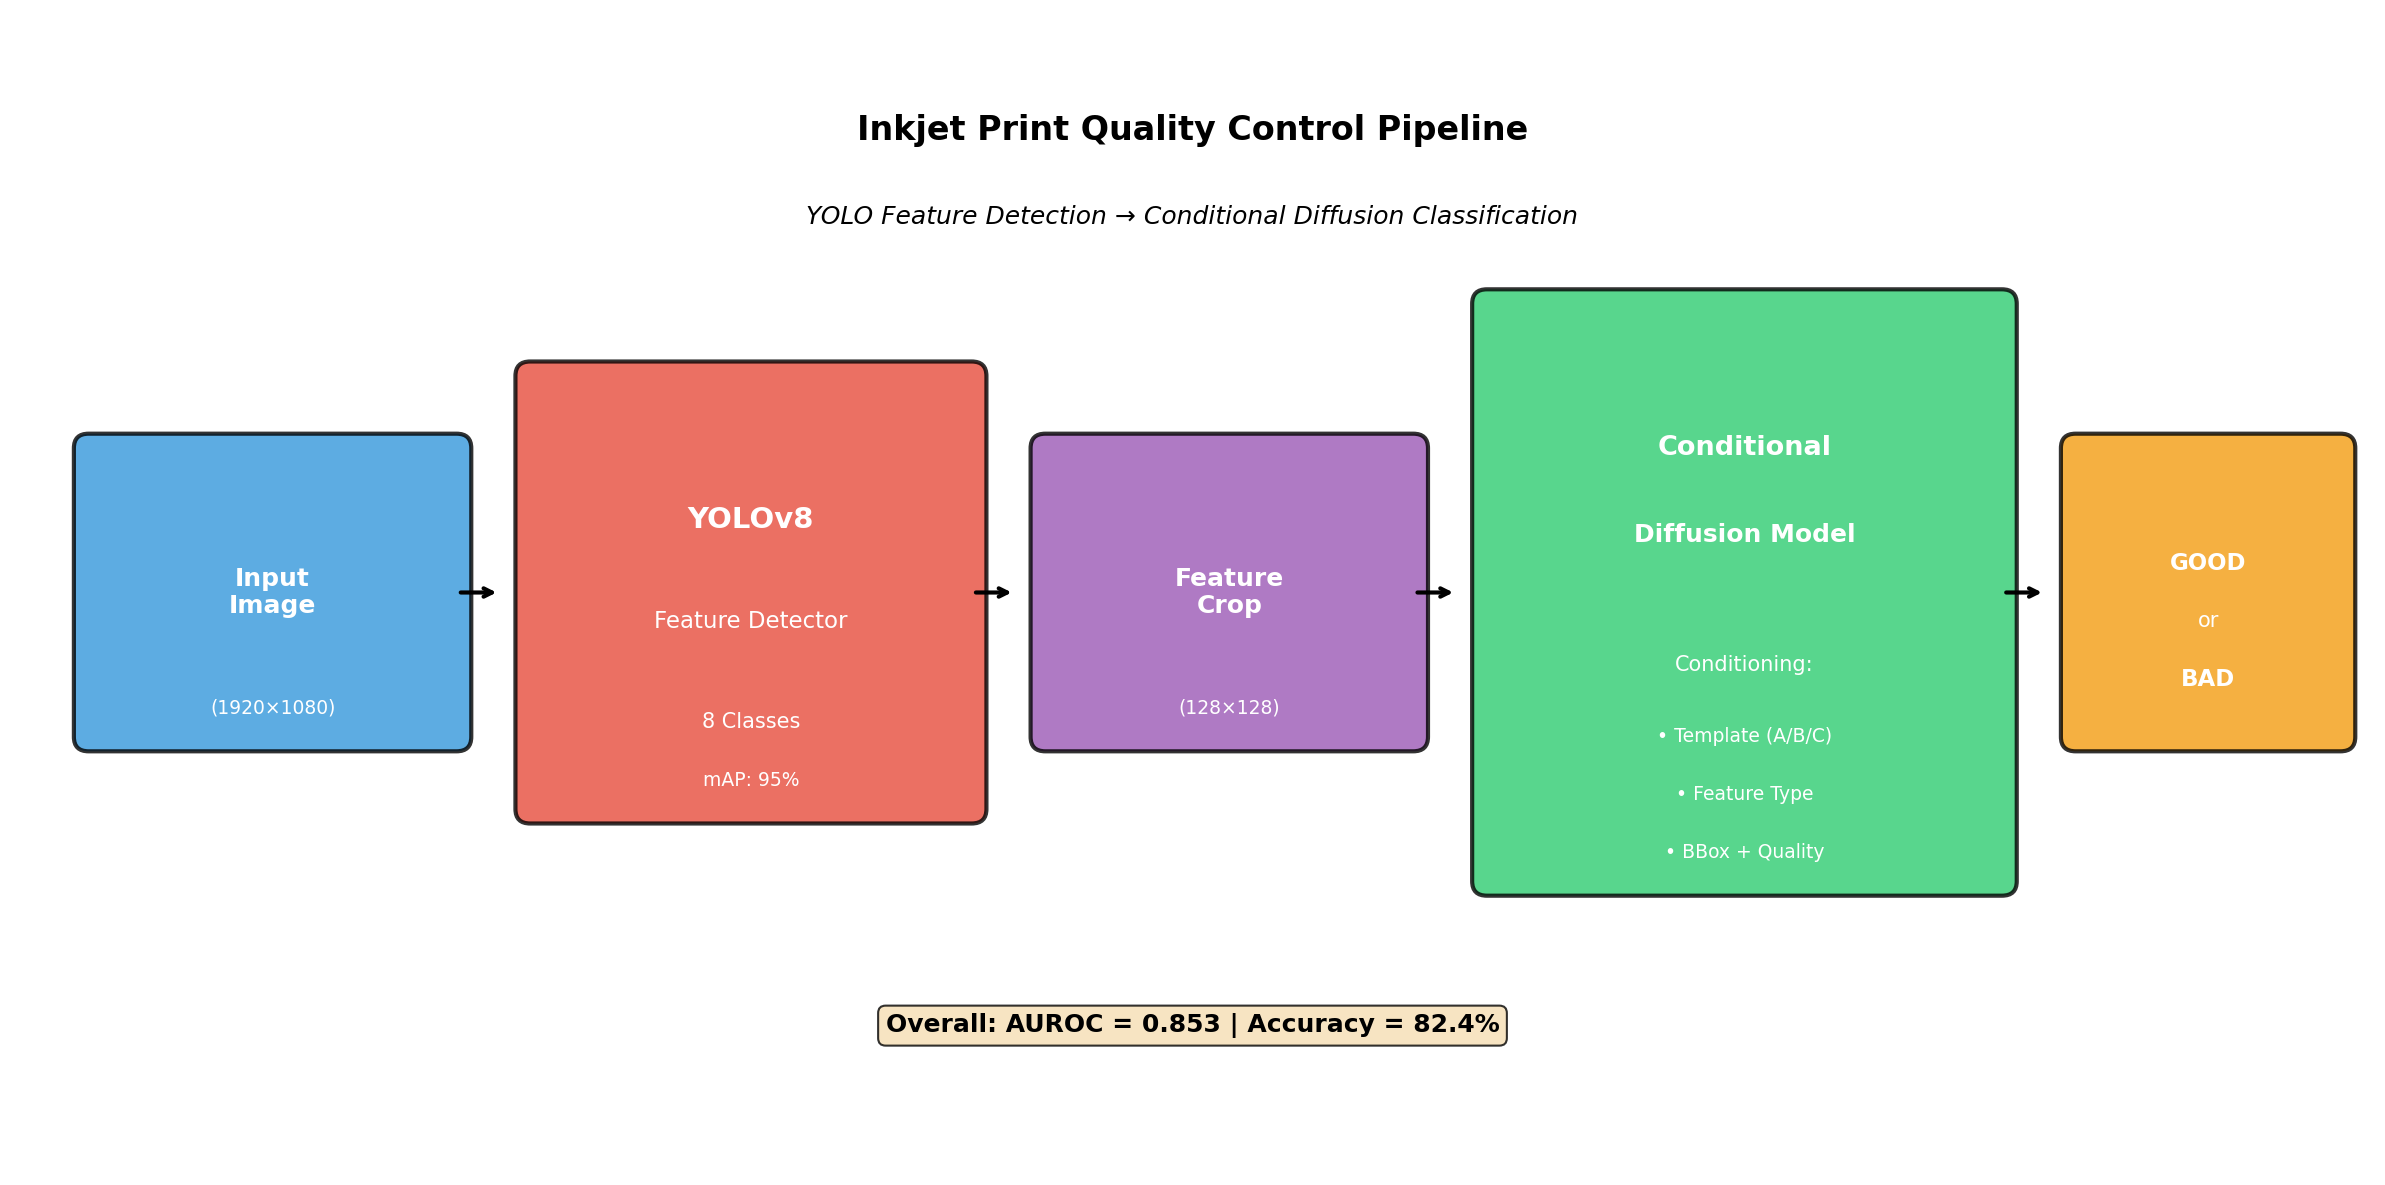
\includegraphics[width=\textwidth]{images/fig_pipeline.png}
    \caption{Two-stage pipeline for inkjet print quality control. Stage~1: YOLOv8 detects and localises individual features on the template image ($1920 \times 1080$). Stage~2: A conditional diffusion model classifies each extracted feature crop ($128 \times 128$) as GOOD or BAD by comparing noise prediction errors under each quality condition.}
    \label{fig:meth:pipeline}
\end{figure}

\textbf{Stage~1 (Feature Detection):} A YOLOv8n model detects and localises 8 types of printed features (angle, dist1, dist6, dots, edge1--edge4) across three template types (A, B, C). Each detection provides a bounding box and feature class, which are used for cropping and conditioning.

\textbf{Stage~2 (Quality Classification):} Each detected feature is cropped, resized to $128 \times 128$ pixels, and classified by the CDM. The model compares noise prediction errors under GOOD and BAD quality conditions to determine the predicted class.


\subsection{Dataset Overview}
\label{sec:meth:inkjet:dataset}

The public FTI\_Zer0P inkjet dataset~\citep{profactor2024fti} contains 1{,}204 inkjet print images from 15 building components, organised into 53 print datasets with up to three print areas per component. Of these images, 960 are labelled as GOOD or BAD for the relevant print-quality features. The retained CDM evaluation uses the labelled images after YOLO-based feature extraction: detections are grouped by 573 source images and expanded into 6{,}408 feature-level crops at $128 \times 128$ pixels across three template types, eight feature types, and binary quality labels (GOOD/BAD). Full dataset statistics, per-feature class balance, and the cross-validation protocol are provided in Section~\ref{sec:exp:inkjet}.
All inkjet experiments in this thesis are evaluated exclusively on the public FTI\_Zer0P dataset~\citep{profactor2024fti}, ensuring full external reproducibility.

\subsection{Multi-Head Conditioning Mechanism}
\label{sec:meth:inkjet:multihead}

The quality classification CDM extends the standard class-conditional diffusion model with a multi-head conditioning mechanism that incorporates four types of metadata simultaneously.

\textbf{Conditioning Inputs:} The model conditions on:
\begin{enumerate}
    \item \textbf{Template type} (categorical, 3 classes): learnt embedding $e_{\text{tmpl}} \in \mathbb{R}^{256}$ implemented as $\text{Embed}(3, 256)$.
    \item \textbf{Feature type} (categorical, 8 classes): learnt embedding $e_{\text{feat}} \in \mathbb{R}^{256}$ implemented as $\text{Embed}(8, 256)$.
    \item \textbf{Quality label} (binary, GOOD/BAD): learnt embedding $e_{\text{qual}} \in \mathbb{R}^{256}$ implemented as $\text{Embed}(2, 256)$.
    \item \textbf{Bounding box} (continuous, 4 values): MLP-encoded embedding $e_{\text{bbox}} \in \mathbb{R}^{256}$ implemented as $\text{MLP}(4 \to 64 \to 256)$.
\end{enumerate}

\textbf{Combination:} All conditioning embeddings in the inkjet pipeline are projected to the same dimensionality (256) and summed:

\begin{equation}
\label{eq:meth:conditioning}
\mathbf{e}_{\mathrm{cond}} = e_{\text{tmpl}} + e_{\text{feat}} + e_{\text{qual}} + e_{\text{bbox}} + e_{\text{time}}
\end{equation}

where $e_{\text{time}}$ is the standard sinusoidal timestep embedding. The combined conditioning vector $\mathbf{e}_{\mathrm{cond}}$ (distinct from the binary class variable $c \in \{0,1\}$ used in the CIFAR-10 OOD formulation) is injected at each UNet resolution level.

\begin{figure}[htbp]
    \centering
    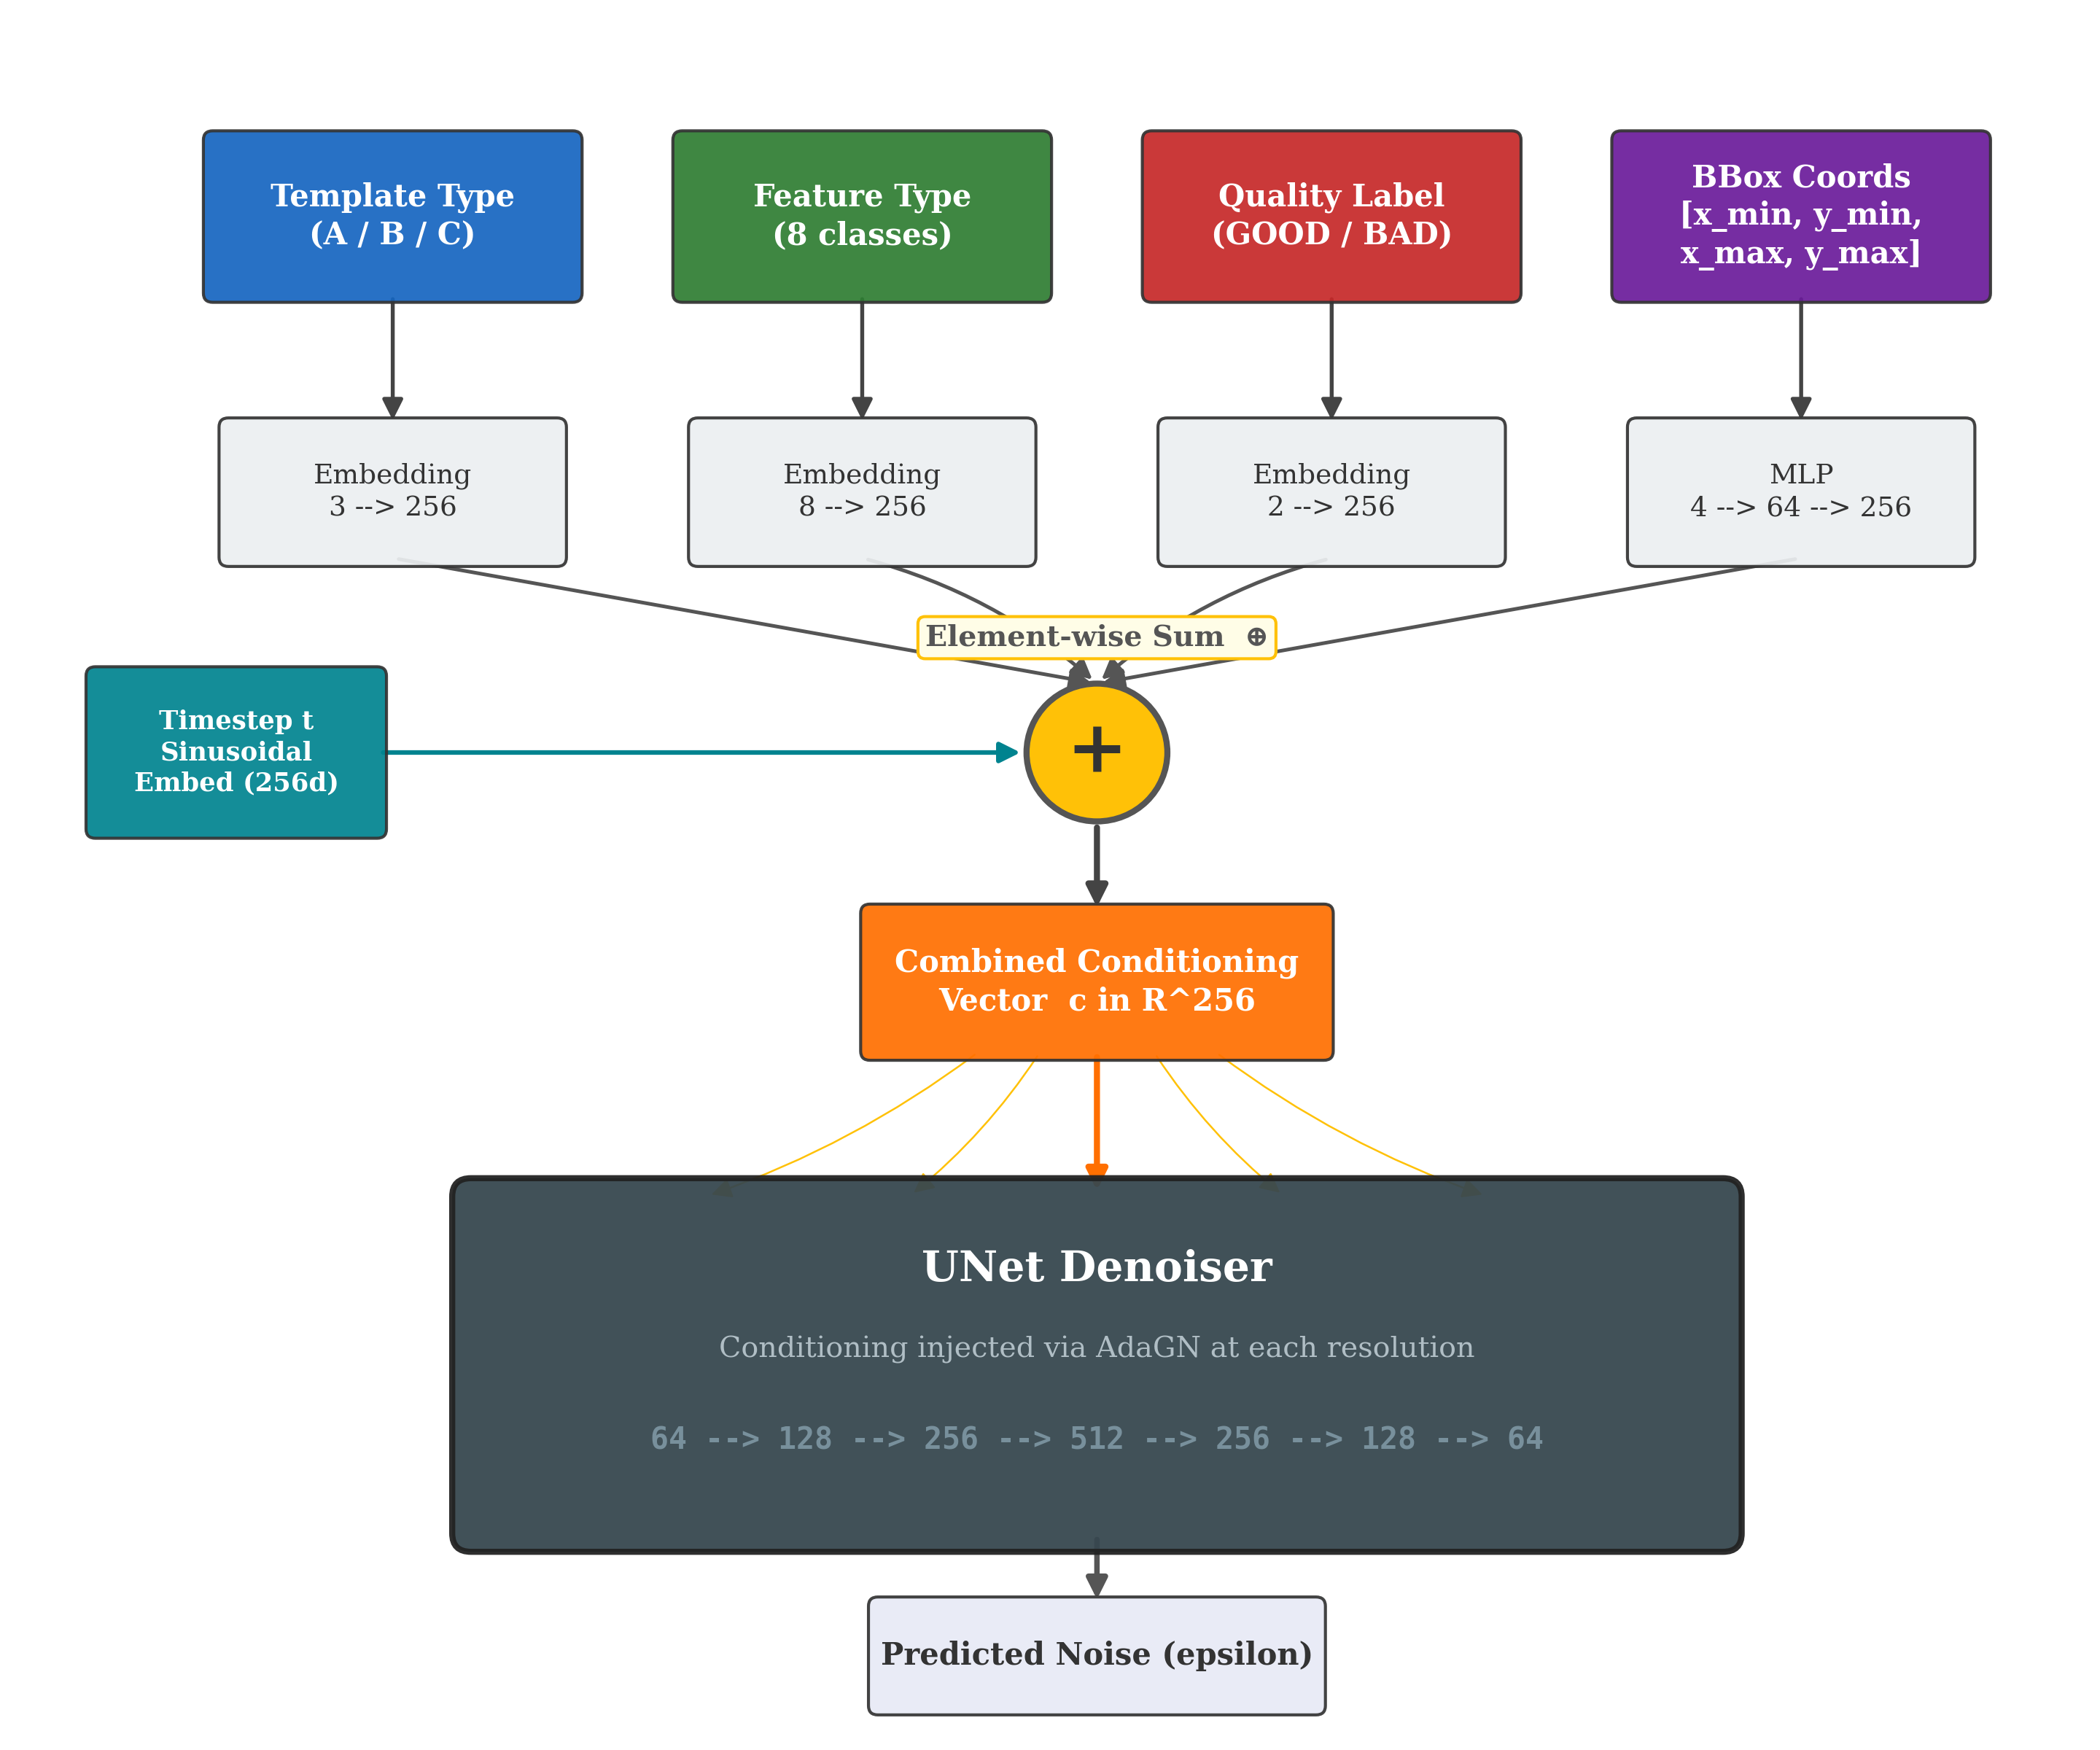
\includegraphics[width=\textwidth]{images/fig_multihead_conditioning.png}
    \caption{Multi-head conditioning mechanism. Four conditioning heads, namely template type ($3 \to 256$), feature type ($8 \to 256$), quality label ($2 \to 256$), and bounding box coordinates ($4 \to 64 \to 256$), are independently encoded and combined via element-wise summation. The resulting conditioning vector is merged with the sinusoidal timestep embedding and injected into the UNet denoiser via Adaptive Group Normalisation (AdaGN) at each resolution level.}
    \label{fig:meth:multihead}
\end{figure}

\textbf{Noise Prediction:} The network predicts noise conditioned on all metadata:

\begin{equation}
\label{eq:meth:noise_pred}
\epsilon_\theta(x_t, t, \text{tmpl}, \text{feat}, \text{qual}, \text{bbox}) = \text{UNet}(x_t, \mathbf{e}_{\mathrm{cond}})
\end{equation}

\subsection{Quality Classification via Differential Noise Prediction}
\label{sec:meth:inkjet:classification}

Classification leverages the CDM's conditional noise prediction to compare how well the model reconstructs each sample under GOOD vs.\ BAD quality assumptions.

\medskip
\noindent\rule{\textwidth}{0.4pt}
\smallskip
\begin{minipage}{\linewidth}\small\sloppy
\noindent\textbf{Algorithm 2} \emph{Quality Classification via Differential Noise Prediction.}\label{alg:quality_classification}

\noindent\textbf{Require:} Feature crop $x \in \mathbb{R}^{3 \times 128 \times 128}$, trained CDM $\epsilon_\theta$\\
\textbf{Require:} Feature metadata: $\text{tmpl}$, $\text{feat}$, $\text{bbox}$\\
\textbf{Require:} Number of Monte Carlo trials $K$, number of timesteps $T$\\
\textbf{Ensure:} Predicted quality $\hat{q} \in \{\text{GOOD}, \text{BAD}\}$, confidence

\noindent\textit{Notation:} $c_g \equiv (\text{tmpl}, \text{feat}, \text{GOOD}, \text{bbox})$;\
$c_b \equiv (\text{tmpl}, \text{feat}, \text{BAD}, \text{bbox})$.

\noindent
1:\ $e_g \leftarrow 0$;\ $e_b \leftarrow 0$\\
2:\ \textbf{for} trial $k = 1$ to $K$ \textbf{do}\\
3:\quad $t_k \sim \text{Uniform}\{1, \ldots, T\}$;\ $\epsilon_k \sim \mathcal{N}(0, I)$\\
4:\quad $x_{t_k} \leftarrow \sqrt{\bar{\alpha}_{t_k}}\, x + \sqrt{1 - \bar{\alpha}_{t_k}}\, \epsilon_k$\\
5:\quad $e_g \leftarrow e_g + \|\epsilon_k - \epsilon_\theta(x_{t_k}, t_k, c_g)\|^2$\\
6:\quad $e_b \leftarrow e_b + \|\epsilon_k - \epsilon_\theta(x_{t_k}, t_k, c_b)\|^2$\\
7:\ \textbf{end for}\\
8:\ $e_g \leftarrow e_g / K$;\ $e_b \leftarrow e_b / K$\\
9:\ \textbf{if} $e_g < e_b$ \textbf{then} $\hat{q} \leftarrow \text{GOOD}$ \textbf{else} $\hat{q} \leftarrow \text{BAD}$\\
10:\ $\text{confidence} \leftarrow |e_g - e_b| / (e_g + e_b)$;\ \textbf{return} $\hat{q}$, confidence
\end{minipage}
\smallskip
\noindent\rule{\textwidth}{0.4pt}
\medskip

\textbf{Key Difference from OOD Detection:} In the OOD detection formulation (Algorithm~1), we use a binary conditional setup ($C = 2$: $c = 0$ for ID, $c = 1$ for OOD), so scoring reduces to a single contrastive comparison via $O(2K)$ forward passes. In quality classification, we similarly compare only two conditions (GOOD vs.\ BAD) while keeping all other conditions (template, feature, bbox) fixed, yielding the same $O(2K)$ cost per sample.

\section{Training Strategies}
\label{sec:meth:training}

Our training procedures incorporate specific loss functions, optimisation strategies, and data augmentation techniques.

\subsection{Loss Functions and Optimisation}
\label{sec:meth:training:loss}

\textbf{Primary Loss:} We use the standard DDPM training objective:

\begin{equation}
\label{eq:meth:ldiffusion}
\mathcal{L}_{\text{diffusion}} = \mathbb{E}_{x,y,t \sim \mathcal{U}[1,T],\,\epsilon \sim \mathcal{N}(0,I)} \left[ \left\| \epsilon - \epsilon_\theta\!\left( \sqrt{\bar{\alpha}_t}\, x + \sqrt{1 - \bar{\alpha}_t}\,\epsilon,\, t,\, y \right) \right\|^2 \right]
\end{equation}

This simple mean squared error (MSE) loss has proven highly effective for training diffusion models.

\textbf{Separation Loss:} To explicitly encourage the model to produce distinct class-conditional noise predictions (and thereby distinct reconstruction error distributions) for ID and OOD conditions, we introduce a contrastive push-apart loss:

\begin{equation}
\label{eq:meth:lsep}
\mathcal{L}_{\text{sep}}(x_t, t) = -\left\| \epsilon_\theta(x_t, t, c{=}0) - \epsilon_\theta(x_t, t, c{=}1) \right\|^2
\end{equation}

where $x_t = \sqrt{\bar{\alpha}_t}\, x + \sqrt{1 - \bar{\alpha}_t}\, \epsilon$ is the noised image obtained via the same forward-diffusion process used by $\mathcal{L}_{\text{diffusion}}$ above, and $\epsilon_\theta(x_t, t, c)$ is the noise predicted by the UNet under class condition $c$. Minimising this term (as part of the total loss) maximises the squared Euclidean distance between class-conditional noise predictions, directly encouraging the model to distinguish ID from OOD inputs at every denoising step. Computing $\mathcal{L}_{\text{sep}}$ requires two additional forward passes of the UNet (one with $c{=}0$ and one with $c{=}1$) beyond the single forward pass already needed for $\mathcal{L}_{\text{diffusion}}$, so each training step performs three forward passes when $\lambda > 0$. In practice this triples the per-step training compute relative to the $\lambda{=}0$ baseline; the explicit per-epoch cost is quantified in Section~\ref{sec:disc:limitations}.

The total training objective combines the diffusion loss with the separation loss:

\begin{equation}
\label{eq:meth:ltotal}
\mathcal{L} = \mathcal{L}_{\text{diffusion}} + \lambda \cdot \mathcal{L}_{\text{sep}}
\end{equation}

where $\lambda \geq 0$ controls the strength of the separation objective. The ablation study in Section~\ref{sec:results:ablations} systematically evaluates $\lambda \in \{0.0, 0.001, 0.01, 0.02, 0.05, 0.1\}$; the final selected CIFAR-10 model uses $\lambda = 0.02$, while the $K$, timestep-sampling, and scoring-strategy ablations use the seed-42 $\lambda=0.01$ checkpoint for compute-budget reasons.

\textbf{Relation to Contrastive Objectives.} The separation loss is structurally related to contrastive training objectives used in representation learning for OOD detection~\cite{tack2020csi, wu2024diffusion}. However, $\mathcal{L}_{\text{sep}}$ differs in two key respects: (i)~it operates in noise-prediction space rather than representation space, directly maximising the gap between class-conditional denoising outputs; and (ii)~it pushes apart predictions from a single shared UNet under different conditioning inputs, rather than training separate encoders or using data augmentation to create contrastive pairs. This design choice is specific to the conditional diffusion framework and enables the separation signal to be injected at the same granularity (per-timestep, per-pixel) as the primary denoising objective.

Because $\mathcal{L}_{\text{sep}}$ is a negative squared norm, it is not bounded below in isolation. The method therefore relies on the denoising objective, small tuned values of $\lambda$, and empirical validation to prevent unproductive norm growth in the two conditional predictions. This risk is one reason we treat $\lambda$ as an ablated hyperparameter rather than a fixed theoretical constant; empirically, the high-weight $\lambda=0.1$ setting drops to 96.67\% Within-CIFAR AUROC, consistent with the separation objective beginning to dominate the denoising loss.

\textbf{Noise Schedule:} For CIFAR-10 experiments, we use a cosine variance schedule as it maintains more signal at higher timesteps compared to linear schedules:

\begin{equation}
\label{eq:meth:cosine_schedule}
\bar{\alpha}_t = \cos^2\!\left( \frac{t/T + s}{1 + s} \cdot \frac{\pi}{2} \right)
\end{equation}

where $s = 0.008$ is a small offset parameter. The retained public inkjet pipeline also uses a cosine noise schedule with $T = 1000$ timesteps, matching the implementation summarised in Chapter~\ref{chap:experimental-setup} and Appendix~\ref{app:experimental-config}.

\subsection{Training Procedure}
\label{sec:meth:training:procedure}

During each training iteration, a batch of images is noised to random timesteps $t \sim \mathcal{U}[1, T]$, the conditional UNet predicts the added noise, and the combined loss $\mathcal{L} = \mathcal{L}_{\text{diffusion}} + \lambda \mathcal{L}_{\text{sep}}$ (Equation~\ref{eq:meth:ltotal}) is minimised via AdamW~\cite{loshchilov2019decoupled} with cosine-annealed learning rate ($\eta = 10^{-4}$, weight decay 0.01, 5-epoch warm-up). An exponential moving average (EMA) of model parameters with decay $\gamma = 0.9999$ is maintained for evaluation. Full training configurations and hyperparameter tables are provided in Chapter~\ref{chap:experimental-setup} and Appendix~\ref{app:experimental-config}.

\subsection{Data Preprocessing}
\label{sec:meth:training:preprocessing}

All images are normalised to $[-1, 1]$ before being passed to the diffusion model. CIFAR-10 images are augmented during training with horizontal flips and random crops (4-pixel padding). Inkjet crops are resized to $128 \times 128$ with no augmentation. Class balancing uses weighted sampling with $w_c = 1/(n_c \cdot C)$. Full preprocessing and augmentation details are provided in Chapter~\ref{chap:experimental-setup}.


\section{Evaluation Framework}
\label{sec:meth:evaluation}

We evaluate using AUROC (probability that a random OOD sample scores higher than a random ID sample; 1.0~$=$~perfect, 0.5~$=$~random) and FPR@95\%TPR (false positive rate at 95\% true positive rate; lower is better) as primary metrics, with AUPRC and Detection Error reported for completeness. Formal definitions are provided in Section~\ref{sec:meth:problem:metrics}.

The threshold $\tau$ is set using Youden's $J$ statistic $\tau^* = \arg\max_\tau[\text{TPR}(\tau) - \text{FPR}(\tau)]$ for balanced scenarios, or at a fixed FPR quantile when controlling false alarm rates. CIFAR-10 reports multi-seed descriptive summaries only for the $\lambda \in \{0.01, 0.02\}$ separation-loss checkpoints; other CIFAR ablations use the documented seed-42 run. Inkjet results use paired $t$-tests and Wilcoxon signed-rank tests with Holm correction over 5~folds.

All models are implemented in PyTorch Lightning with Hydra-based configuration; full implementation details are covered in Chapter~\ref{chap:implementation}.
\endgroup
